\documentclass[10pt]{armath}
\usepackage{amsmath}
\usepackage{amsthm}
\usepackage{csquotes}
\usepackage{enumitem}
\usepackage{subcaption}
\usepackage{todonotes}
\usepackage[utf8]{inputenc}
\usepackage[english]{babel}
\usepackage{multicol}
\usepackage{tikz}
\usepackage{pgfplots}
\usepackage{subfiles}
\usepackage{algpseudocode}
\usepackage{algorithm}
\usepackage{graphics}
\usepackage{longtable}
\usepackage{fontawesome}
\usepackage[toc,page]{appendix}
\usepackage[hidelinks]{hyperref}
\usepackage{minted}
\usepackage[margin=1in]{geometry}
\usetikzlibrary{calc,patterns,angles,quotes,positioning}
\setminted[lua]{
  linenos=true,
  frame=lines,
  framesep=5pt,
  fontsize=\footnotesize
}

\numberwithin{equation}{section}
\newenvironment{Figure}
{\par\medskip\noindent\minipage{\linewidth}}
{\endminipage\par\medskip}

\theoremstyle{definition}
\newtheorem{example}{Example}[section]
\newtheorem{definition}{Definition}[section]

\renewcommand{\thealgorithm}{\arabic{section}.\arabic{algorithm}}
\renewcommand\thefigure{\thesection.\arabic{figure}}

\newcommand{\N}{\mathbb{N}}
\newcommand{\R}{\mathbb{R}}
\newcommand{\K}{\mathcal{K}}
\newcommand{\ep}{{\varepsilon}}

\newcommand{\pder}[2]{\frac{\partial #1}{\partial #2}}
\newcommand{\ppder}[2]{\frac{\partial^2 #1}{\partial {#2}^2}}
\newcommand{\px}{{\partial x}}
\newcommand{\ph}{\varphi}
\newcommand{\e}{{(e)}}
\newcommand{\wt}[1]{\widetilde{#1}}
\newcommand{\wb}[1]{\overline{#1}}
\newcommand{\braket}[2]{\left<{#1},{#2}\right>}
\newcommand{\pluseq}{\mathrel{+}=}
\newcommand{\minuseq}{\mathrel{-}=}
\newcommand{\ra}{\rightarrow}
\newcommand{\lra}{\leftrightarrow}

\newcommand{\hdiv}[3]{
  \vspace{#1}%
  \noindent\rule{\textwidth}{#2}%
  \vspace{#3}%
}
\newcommand{\code}[2]{
  \begin{figure}[thp]\centering\begin{minipage}{0.8\textwidth}\inputminted{#1}{#2}\end{minipage}\end{figure}
}

\title{Physicaly Based Rendering}
\author{Arden Rasmussen}
\date{\today}

\begin{document}
\maketitle

\begin{multicols}{2}
  \section{Introduction}%
  \label{sec:introduction}

  \section{Radiometry \& Light Attenuation}%
  \label{sec:radiometry_&_light_attenuation}

  \subsection{Radiometry Recap}%
  \label{sub:radiometry_recap}

  \textbf{What to measure in a simulation?}

  \begin{definition}[Radiant flux]
    Total amount of energy passing thought surface (measured per second).
    $\Phi\left[W\right]$.
  \end{definition}

  This is not sufficient to measure, because it is the energy per surface area,
  then consider a large radiant flux that could either be
  \begin{enumerate}
    \item a lot of energy over a small surface.
    \item a little energy over a large surface.
  \end{enumerate}

  Thus this metric is too ambiguous, and not good enough for us.

  \begin{definition}[Irradiance]
    Total amount of energy passing through a unit area. $E\left[W/m^2\right]$.
  \end{definition}

  This is still ambiguous, we haven't fixed the angle which the light arrives to the
  surface. So
  \begin{enumerate}
    \item a lot of energy in a huge angle
    \item a little energy in a small angle
  \end{enumerate}
  will measure the same irradiance.

  \begin{definition}[Radiance]
    Total energy passing through a unit area with unit angle
    $I\left[W/\left(m^2\cdot sr\right)\right]$\footnote{Angle in more dimensions
      is called solid angle, for which the unit is steradians($sr$)}.
  \end{definition}

  This is the measurement that we will be using.

  \subsection{The most fundamental question}%
  \label{sub:the_most_fundamental_question}

  \textbf{How much light exits a surface point in a given direction?}

  The complete answer is given by Maxwell equations! In practice, we don't do
  this, it would require simulations on the size of wavelengths of light, and
  that is overly complex.

  The real solution is the rendering equation!

  \subsection{The scalar product}%
  \label{sub:the_scalar_product}

  \begin{align*}
    \vec{a}\cdot\vec{b}\equiv||\vec{a}||\cdot||\vec{b}||\cos\theta.
  \end{align*}

  For this work we will always assume that the vectors are normalized, and so
  this becomes

  \begin{align*}
    \vec{a}\cdot\vec{b}\equiv\cos\theta.
  \end{align*}

  \subsection{Terminology}%
  \label{sub:terminology}

  The key components in the terminology are depicted in figure
  \ref{fig:02_1}\footnote{Vectors are always pointing away from the point of
    intrest $x$}.

  \begin{Figure}
    \begin{center}
      \documentclass[tikz,border=10pt,convert]{standalone}
\usepackage{fontawesome}
\usetikzlibrary{calc,patterns,angles,quotes,positioning}

\begin{document}
\begin{tikzpicture}
  \coordinate (O) at (0,0);
  \coordinate (A) at (-5,5);
  \coordinate (B) at (5,5);
  \coordinate (S) at (0,5);
  \draw[->,>=stealth] (O) -- (A);
  \draw[->,>=stealth] (O) -- (B);
  \draw[->,>=stealth] (O) -- (S);
  \draw (-5,0) -- (5,0);

  \pic [draw, -, "$\theta_i$", angle eccentricity=1.5] {angle = S--O--A};
  \pic [draw, -, "$\theta_r$", angle eccentricity=1.5] {angle = B--O--S};


  \node[above] at (A) {$\vec{V}$};
  \node[above] at (B) {$\vec{V}'$};
  \node[below] at (O) {$x$};
  \node[right] at (S) {$\vec{L}$,$\vec{R}$};
  \node[left] at (S) {$\vec{N}$};
  \node[above] at (S) {\faSunO};
\end{tikzpicture}
\end{document}

    \end{center}
    \captionof{figure}{Basic terminology}
    \label{fig:02_1}
  \end{Figure}

  \begin{enumerate}
    \item[$\vec{V}$] direction towards the viewer (eye,camera)
    \item[$\vec{N}$] surface normal
    \item[$\vec{L}$] vector point towards the light source
    \item[$\vec{R}$] reflected ray direction
      $\vec{R}=\vec{L}-2\vec{N}\left(\vec{L}\cdot\vec{N}\right)$.
    \item[$\theta_i,\theta_r$] incident and reflected angles.
  \end{enumerate}

  \subsection{Light Attenuation}%
  \label{sub:light_attenuation}

  When the sun is directly above as in figure \ref{fig:02_1}, then
  \begin{align*}
    \left(\vec{L}\cdot\vec{N}\right)\Phi=\cos\alpha|_{\alpha\approx0}\Phi=\Phi.
  \end{align*}

  \begin{Figure}
    \begin{center}
      \documentclass[tikz,border=10pt,convert]{standalone}
\usepackage{fontawesome}
\usetikzlibrary{calc,patterns,angles,quotes,positioning}

\begin{document}
\begin{tikzpicture}
  \coordinate (O) at (0,0);
  \coordinate (A) at (-5,5);
  \coordinate (B) at (5,5);
  \coordinate (N) at (0,5);
  \coordinate (S) at (3,5);
  \coordinate (SI) at (-3,5);
  \draw[->,>=stealth] (O) -- (A);
  \draw[->,>=stealth] (O) -- (B);
  \draw[->,>=stealth] (O) -- (N);
  \draw[->,>=stealth] (O) -- (S);
  \draw[->,>=stealth] (O) -- (SI);
  \draw (-5,0) -- (5,0);

  \pic [draw, -, "$\theta_i$", angle eccentricity=1.5] {angle = N--O--A};
  \pic [draw, -, "$\theta_r$", angle eccentricity=1.5] {angle = B--O--N};
  \pic [draw, -, "$\alpha$", angle eccentricity=1.5, angle radius=1cm] {angle = S--O--N};


  \node[above] at (A) {$\vec{V}$};
  \node[above] at (B) {$\vec{V}'$};
  \node[below] at (O) {$x$};
  \node[right] at (S) {$\vec{L}$};
  \node[above] at (S) {\faSunO};
  \node[right] at (SI) {$\vec{R}$};
  \node[left] at (N) {$\vec{N}$};
\end{tikzpicture}
\end{document}

    \end{center}
    \captionof{figure}{Light attenuation with sun at $45^\circ$.}
    \label{fig:02_2}
  \end{Figure}

  When the sun is at an angle as in figure \ref{fig:02_2}, then
  \begin{align*}
    \left(\vec{L}\cdot\vec{N}\right)\Phi=\cos\alpha|_{\alpha\approx45^\circ}\Phi=0.7\Phi.
  \end{align*}

  \begin{Figure}
    \begin{center}
      \documentclass[tikz,border=10pt,convert]{standalone}
\usepackage{fontawesome}
\usetikzlibrary{calc,patterns,angles,quotes,positioning}

\begin{document}
\begin{tikzpicture}
  \coordinate (O) at (0,0);
  \coordinate (A) at (-5,5);
  \coordinate (B) at (5,5);
  \coordinate (N) at (0,5);
  \coordinate (S) at (5,1);
  \coordinate (SI) at (-5,1);
  \draw[->,>=stealth] (O) -- (A);
  \draw[->,>=stealth] (O) -- (B);
  \draw[->,>=stealth] (O) -- (N);
  \draw[->,>=stealth] (O) -- (S);
  \draw[->,>=stealth] (O) -- (SI);
  \draw (-5,0) -- (5,0);

  \pic [draw, -, "$\theta_i$", angle eccentricity=1.5] {angle = N--O--A};
  \pic [draw, -, "$\theta_r$", angle eccentricity=1.5] {angle = B--O--N};
  \pic [draw, -, "$\alpha$", angle eccentricity=1.5, angle radius=1cm] {angle = S--O--N};


  \node[above] at (A) {$\vec{V}$};
  \node[above] at (B) {$\vec{V}'$};
  \node[below] at (O) {$x$};
  \node[right] at (S) {$\vec{L}$};
  \node[above] at (S) {\faSunO};
  \node[right] at (SI) {$\vec{R}$};
  \node[left] at (N) {$\vec{N}$};
\end{tikzpicture}
\end{document}

    \end{center}
    \captionof{figure}{Light attenuation with sun at $90^\circ$.}
    \label{fig:02_3}
  \end{Figure}

  When the sun is at an angle as in figure \ref{fig:02_3}, then
  \begin{align*}
    \left(\vec{L}\cdot\vec{N}\right)\Phi=\cos\alpha|_{\alpha\approx90^\circ}\Phi=0.
  \end{align*}

  Thus we can model this light attenuation using this dot product.

  \section{BRDF models \& The Rendering Equation}%
  \label{sec:brdf_models_&_the_rendering_equation}

  \subsection{Materials}%
  \label{sub:materials}

  \textbf{What makes the difference between materials?}

  Different materials reflect incoming light to different directions and absorb
  different amounts of it.

  \begin{Figure}
    \begin{center}
      \centering
      \begin{minipage}{0.3\textwidth}
        \begin{center}
          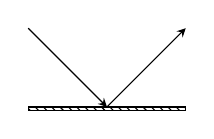
\begin{tikzpicture}[scale=0.2]
  \coordinate (S) at (-5,5);
  \coordinate (O) at (0,0);
  \draw[->,>=stealth] (S) -- (O);
  \draw[->,>=stealth] (O) -- (5,5);
  \draw[pattern=north west lines] (-5,0) rectangle (5,-0.2);
\end{tikzpicture}

          Specular
        \end{center}
      \end{minipage}
      \begin{minipage}{0.3\textwidth}
        \begin{center}
          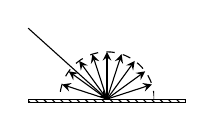
\begin{tikzpicture}[scale=0.2]
  \coordinate (S) at (-5,4.5);
  \coordinate (O) at (0,0);
  \draw[->,>=stealth] (S) -- (O);
  \draw[->,>=stealth] (O) -- (2.853,0.927);
  \draw[->,>=stealth] (O) -- (2.427,1.763);
  \draw[->,>=stealth] (O) -- (1.763,2.427);
  \draw[->,>=stealth] (O) -- (0.927,2.853);
  \draw[->,>=stealth] (O) -- (-2.853,0.927);
  \draw[->,>=stealth] (O) -- (-2.427,1.763);
  \draw[->,>=stealth] (O) -- (-1.763,2.427);
  \draw[->,>=stealth] (O) -- (-0.927,2.853);
  \draw[->,>=stealth] (O) -- (0, 3);
  \begin{scope}
    \clip (-3,0) rectangle (3,3);
    \draw[dashed] (0,0) circle (3);
  \end{scope}
  \draw[pattern=north west lines] (-5,0) rectangle (5,-0.2);
\end{tikzpicture}

          Diffuse
        \end{center}
      \end{minipage}
      \begin{minipage}{0.3\textwidth}
        \begin{center}
          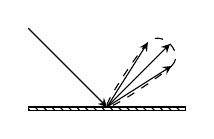
\begin{tikzpicture}[scale=0.2]
  \coordinate (S) at (-5,5);
  \coordinate (O) at (0,0);
  \coordinate (A) at (4.1,2.6);
  \coordinate (B) at (2.6,4.1);
  \draw[->,>=stealth] (S) -- (O);
  \draw[->,>=stealth] (O) -- (4,4);
  \draw[->,>=stealth] (O) -- (A);
  \draw[->,>=stealth] (O) -- (B);
  \draw[dashed] plot [smooth cycle] coordinates { (O) (A) (4,4) (B) };
  \draw[pattern=north west lines] (-5,0) rectangle (5,-0.2);
\end{tikzpicture}

          Glossy
        \end{center}
      \end{minipage}
    \end{center}
    \captionof{figure}{Specula, diffuse, and spread reflections from a surface}
    \label{fig:03_1}
  \end{Figure}


  \begin{description}
    \item[Specular] For one incoming direction there is only one outgoing
      direction, this is what a mirror would be.
    \item[Diffuse] For one incoming direction on there are many possible
      outcomes.
    \item[Glossy/Spread] This is a mixture of specular and diffuse.
  \end{description}

  \subsection{BRDF}%
  \label{sub:brdf}

  We will create a probability density function that takes
  \begin{enumerate}
    \item an incoming light direction
    \item a point on the surface
  \end{enumerate}
  as parameters, and outputs the probability of a given outward direction. We
  define this function as

  \begin{definition}[Bidirectional reflectance distribution function(BRDF)]
    \begin{align*}
      f_r\left(\vec{\omega},x,\vec{\omega}'\right).
    \end{align*}
  \end{definition}

  What about materials that don't reflect all incoming light, some things that
  could transmit the light. There are some examples in figure \ref{fig:03_2}.

  \begin{Figure}
    \begin{center}
      \centering
      \begin{minipage}{0.3\textwidth}
        \begin{center}
          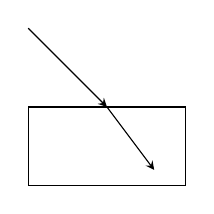
\begin{tikzpicture}[scale=0.2]
  \coordinate (S) at (-5,5);
  \coordinate (O) at (0,0);
  \draw[->,>=stealth] (S) -- (O);
  \draw[->,>=stealth] (O) -- (3,-4);
  \draw (-5,0) rectangle (5,-5);
\end{tikzpicture}

          Specular
        \end{center}
      \end{minipage}
      \begin{minipage}{0.3\textwidth}
        \begin{center}
          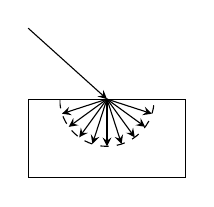
\begin{tikzpicture}[scale=0.2]
  \coordinate (S) at (-5,4.5);
  \coordinate (O) at (0,0);
  \draw[->,>=stealth] (S) -- (O);
  \draw[->,>=stealth] (O) -- (2.853,-0.927);
  \draw[->,>=stealth] (O) -- (2.427,-1.763);
  \draw[->,>=stealth] (O) -- (1.763,-2.427);
  \draw[->,>=stealth] (O) -- (0.927,-2.853);
  \draw[->,>=stealth] (O) -- (-2.853,-0.927);
  \draw[->,>=stealth] (O) -- (-2.427,-1.763);
  \draw[->,>=stealth] (O) -- (-1.763,-2.427);
  \draw[->,>=stealth] (O) -- (-0.927,-2.853);
  \draw[->,>=stealth] (O) -- (0, -3);
  \begin{scope}
    \clip (-3,0) rectangle (3,-3);
    \draw[dashed] (0,0) circle (3);
  \end{scope}
  \draw (-5,0) rectangle (5,-5);
\end{tikzpicture}

          Diffuse
        \end{center}
      \end{minipage}
      \begin{minipage}{0.3\textwidth}
        \begin{center}
          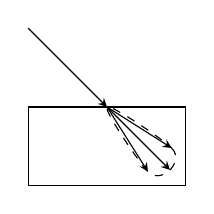
\begin{tikzpicture}[scale=0.2]
  \coordinate (S) at (-5,5);
  \coordinate (O) at (0,0);
  \coordinate (A) at (4.1,-2.6);
  \coordinate (B) at (2.6,-4.1);
  \draw[->,>=stealth] (S) -- (O);
  \draw[->,>=stealth] (O) -- (4,-4);
  \draw[->,>=stealth] (O) -- (A);
  \draw[->,>=stealth] (O) -- (B);
  \draw[dashed] plot [smooth cycle] coordinates { (O) (A) (4,-4) (B) };
  \draw (-5,0) rectangle (5,-5);
\end{tikzpicture}

          Glossy
        \end{center}
      \end{minipage}
    \end{center}
    \captionof{figure}{Transmitted models of light}
    \label{fig:03_2}
  \end{Figure}

  Things are transparent because atom are mostly empty. Things are opaque,
  because the electrons are absobing the photons. The electrons then jump to an
  outer orbit. Glass is transparent because the orbits of the electrons are too
  far apart, so that if an electron absorbs a photon it does not get enough
  energy to jump to the higher orbit. Note that if the light is of a higher
  energy (not in the visible spectrum) then it could be opaque. For instance
  glass is opaque to UV-light.

  \subsection{BTDF}%
  \label{sub:btdf}

  For light that is also transmited, we have the Bidirectional transmittance
  distribution function.

  \begin{Figure}
    \begin{center}
      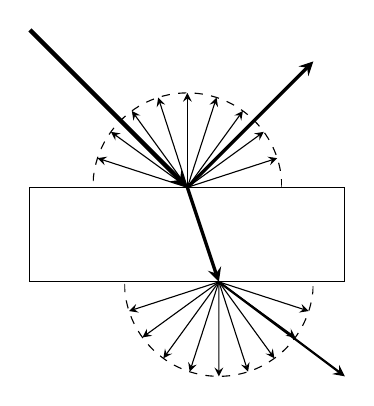
\begin{tikzpicture}[scale=0.4]
  \coordinate (S) at (-5,5);
  \coordinate (O) at (0,0);
  \coordinate (OT) at (1,-3);
  \draw[->,>=stealth,ultra thick] (S) -- (O);
  \draw[->,>=stealth,very thick] (O) -- (4,4);
  \draw[->,>=stealth] (O) -- (2.853,0.927);
  \draw[->,>=stealth] (O) -- (2.427,1.763);
  \draw[->,>=stealth] (O) -- (1.763,2.427);
  \draw[->,>=stealth] (O) -- (0.927,2.853);
  \draw[->,>=stealth] (O) -- (-2.853,0.927);
  \draw[->,>=stealth] (O) -- (-2.427,1.763);
  \draw[->,>=stealth] (O) -- (-1.763,2.427);
  \draw[->,>=stealth] (O) -- (-0.927,2.853);
  \draw[->,>=stealth] (O) -- (0, 3);
  \begin{scope}
    \clip (-3,0) rectangle (3,3);
    \draw[dashed] (O) circle (3);
  \end{scope}

  \draw[->,>=stealth,very thick] (O) -- (OT);

  \draw[->,>=stealth,thick] (OT) -- (5,-6);
  \draw[->,>=stealth] (OT) -- (3.853,-3.927);
  \draw[->,>=stealth] (OT) -- (3.427,-4.763);
  \draw[->,>=stealth] (OT) -- (2.763,-5.427);
  \draw[->,>=stealth] (OT) -- (1.927,-5.853);
  \draw[->,>=stealth] (OT) -- (-1.853,-3.927);
  \draw[->,>=stealth] (OT) -- (-1.427,-4.763);
  \draw[->,>=stealth] (OT) -- (-0.763,-5.427);
  \draw[->,>=stealth] (OT) -- (0.073,-5.853);
  \draw[->,>=stealth] (OT) -- (1, -6);
  \begin{scope}
    \clip (-2,-3) rectangle (4,-6);
    \draw[dashed] (OT) circle (3);
  \end{scope}
  \draw (-5,0) rectangle (5,-3);
\end{tikzpicture}

    \end{center}
    \captionof{figure}{Light that is both reflected and transmitted}
    \label{fig:03_3}
  \end{Figure}

  \subsection{BSDF}%
  \label{sub:bsdf}

  To generalize the BRDF and BTDF, we use the BSDF (S is for scattering).

  \subsection{BRDF Properties}%
  \label{sub:brdf_properties}

  \begin{enumerate}
    \item Helmholtz-reciprocity: The direction of the ray of light can be
      reversed
      \begin{align*}
        \forall\vec{\omega},\vec{\omega}':\quad
        f_r\left(\vec{\omega},x,\vec{\omega}'\right)=f_r\left(\vec{\omega}',x,\vec{\omega}\right)
      \end{align*}
    \item Positivity: It is an impossibility for an exit direction to have a
      negative probability.
      \begin{align*}
        \forall\vec{\omega},\vec{\omega}':\quad
        f_r\left(\vec{\omega},x,\vec{\omega}'\right)\geq 0
      \end{align*}
    \item Energy conservation: An object may reflect or absorb incoming light,
      but no more can com out than the incoming amount.
      \begin{align*}
        \int_\Omega
        f_r\left(\vec{\omega},x,\vec{\omega}'\right)\cos\theta d\vec{\omega}'\leq
        1
      \end{align*}
      This means that we add up all the incoming energy from all possible
      directions, taking the light attenuation into account. If it equals 1, all
      light is is reflected, if it is less than 1 some of the light is absorbed.
      More than 1 is impossible.
  \end{enumerate}

  \subsection{The Rendering Equation}%
  \label{sub:the_rendering_equation}

  An object can emit light itself. It also receives light form different
  directions, which it will either reflect or absorb, therefore

  \begin{Figure}
    \begin{center}
      \begin{tikzpicture}[scale=1]
  \coordinate (O) at (0,0);
  \coordinate (E) at (-2,2);
  \coordinate (I) at (2,2);
  \node[left] at (E) {\faEye};
  \draw[fill] (O) circle [radius=0.02] node[below]{$x$};
  \draw (2,0) arc (0:-180:2 and 0.6);
  \draw[dashed] (2,0) arc (0:180:2 and 0.6);
  \draw (2,0) arc (0:180:2 and 2) node[midway,above]{$\Omega$};
  \draw[->,>=stealth,thick] (O) -- (E) node[above]{$w_o$};
  \draw[->,>=stealth,thick] (O) -- (I) node[above]{$w_i$};
  \draw[->,>=stealth] (2,1) -- (O);
  \draw[->,>=stealth] (1,2) -- (O);
\end{tikzpicture}

    \end{center}
    \captionof{figure}{Rendering Equation Representation}
    \label{fig:03_3}
  \end{Figure}

  \begin{align*}
    L_o\left(x,\vec{\omega}\right)=\underbrace{L_e\left(x,\vec{\omega}\right)}_\text{emitted}+\underbrace{\int_\Omega
      L_i\left(x,\vec{\omega}\right)f_r\left(\vec{\omega},x,\vec{\omega}'\right)\cos\theta
      d\vec{\omega}'}_\text{reflected incoming light}
  \end{align*}

  Where
  \begin{description}
    \item[$L_o\left(x,\vec{\omega}\right)$] exiting radiance in point $x$ towards
      direction $\vec{\omega}$.
    \item[$L_e\left(x,\vec{\omega}\right)$] emitted radiance in point $x$ towards
      direction $\vec{\omega}$.
    \item[$\int_\Omega\cdots d\vec{\omega}'$] Sum of the incoming radiance from
      all $\vec{\omega}'$ directions\footnote{$\Omega$ is only the hemisphere,
        because the $\cos\theta$ from below would be negative, and we don't need
        to deal with this light}.
    \item[$L_i\left(x,\vec{\omega}'\right)$] Incoming radiance from the direction
      $\vec{\omega}'$ to point $x$.
    \item[$f_r\left(\vec{\omega},x,\vec{\omega}'\right)$] BRDF.
    \item[$\cos\theta$] light attenuation.
  \end{description}

  Difficulties
  \begin{enumerate}
    \item The exitant radiance of a point $x$ depends on the incoming radiance of
      every other point, which also depend on $x$. Thus every point depends on
      every other point, and so would be infinitely recursive.
    \item It is absolutely hopeless to compute this integral in closed form.
    \item The integral is also infinite-dimensional. We need to compute an
      infinite number of bounces of light.
    \item It is often singular.
  \end{enumerate}

  As of now, we have insufficient knowledge to even give an approximate solution
  to this equation.

  The solution is to compute the entirety of the light path, then move the last
  bounce point, and compute the contribution of each individual light source to
  the sensor. This is not what we will be using. But here it is
  \begin{align*}
    L_o\left(p'\ra p\right)&=L_e\left(p'\ra p\right)\\&+\int_AL_i\left(p^n\ra
      p'\right)f_r\left(p^n\ra p'\ra p\right)\\&\quad\quad\cdot G\left(p^n\lra
      p'\right)dA\left(p^n\right)
  \end{align*}
  \begin{description}
    \item[$L_o\left(p'\ra p\right)$] outgoing radiance from point $p'$ to $p$.
    \item[$L_e\left(p'\ra p\right)$] emitted radiance from $p'$ to $p$.
    \item[$\int_\Omega\cdots dA\left(p^n\right)'$] sum for all possible $p^n$
      surface points.
    \item[$L_i\left(p^n\ra p'\right)$] incoming radiance form point $p^n$ to
      $p'$.
    \item[$f_r\left(p^n\ra p'\ra p\right)$] probability of $p^n\ra p'\ra p$
      transfer.
    \item[$G\left(p^n\lra p'\right)$] geometry term.
  \end{description}

  \section{Diffuse, Specular, and Ambient Shading}%
  \label{sec:diffuse_specular_and_ambient_shading}

  \subsection{BRDF types}%
  \label{sub:brdf_types}

  Illumination model for \textit{ambient} BRDF(simplified):
  \begin{align*}
    I=k_aI_a
  \end{align*}
  \begin{description}
    \item[$k_a$] ambient coefficient of an object.
    \item[$I_a$] ambient intensity of the scene/light source.
  \end{description}

  Illumination model for \textit{diffuse} BRDF(simplified);
  \begin{align*}
    I=k_d\left(\vec{L}\cdot\vec{N}\right)
  \end{align*}
  \begin{description}
    \item[$k_d$] diffuse coefficient of an object\footnote{The diffuse and other
        coefficients may take different values for different wavelengths. An
        object may absorb most of the green light, but may reflect all incoming
        red light in the meantime. The proper term would be $k_{d,\lambda}$.}
    \item[$\vec{L}$] vector point to the light source
    \item[$\vec{N}$] surface normal
  \end{description}

  Illumination model for \textit{specular} BRDF(simplified):
  \begin{align*}
    I=k_s{\left(\vec{V}\cdot\vec{R}\right)}^n
  \end{align*}
  \begin{description}
    \item[$k_s$] specular coefficient of an object
    \item[$\vec{V}$] vector pointing to the viewer/camera
    \item[$\vec{R}$] reflected direction of the light ray
    \item[${\left(\cdot\right)}^n$] shininess factor.
  \end{description}
  The view vector is in the formula, therefor it should look differently if we
  turn out heads.

  The sum of these three type of illumination model is called Phong shading, and
  is a descriptive representation of the shading.

  \subsection{The Illumination Equation}%
  \label{sub:the_illumination_equation}

  This is the simplification of the rendering equation
  \begin{align*}
    I=k_aI_a+I_i\left(k_d\left(\vec{L}\cdot\vec{N}\right)+k_s{\left(\vec{V}\cdot\vec{R}\right)}^n\right)
  \end{align*}
  \begin{itemize}
    \item Only accounts for the direct illumination of the light sources.
    \item The indirect illumination is neglected, the ambient term helps to
      reinject some of the lost energy into the system.
    \item This is indeed a very crude approximation of physically reality.
  \end{itemize}

  This could be summed for all light sources, we kept this notation for
  simplicity.

  Something is missing, what is missing?

  \subsection{The Algorithm}%
  \label{sub:the_algorithm}

  \begin{enumerate}
    \item Construction of the camera/eye rays
    \item Intersection with the scene object
    \item Shading
    \item Reflection/refraction directions
    \item Recursion
  \end{enumerate}

  The ray doesn't stop at the first intersection, we have to trace it further
  as it will either get reflected or refracted.

  \section{The Fresnel Equation and Schlick's Approximation}%
  \label{sec:the_fresnel_equation_and_schlick_s_approximation}

  \begin{Figure}
    \begin{center}
      \begin{tikzpicture}[scale=0.4]
  \coordinate (O) at (0,0);
  \coordinate (S) at (-5,3);
  \coordinate (RE) at (5,3);
  \coordinate (RF) at (2,-3);
  \coordinate (N) at (0,3);
  \coordinate (NN) at (0,-3);
  \draw[->,>=stealth,thick] (O) -- (S);
  \draw[->,>=stealth] (O) -- (RE) node[right]{Reflection};
  \draw[->,>=stealth,thick] (O) -- (RF) node[right]{Refraction};
  \draw (NN)node[left]{$-\vec{N}$} -- (O) -- (N)node[left]{$\vec{N}$};

  \pic [draw, -, "$\theta_i$", angle eccentricity=1.5] {angle = N--O--S};
  \pic [draw, -, "$\theta_r$", angle eccentricity=1.5] {angle = RE--O--N};
  \pic [draw, -, "$\theta_t$", angle eccentricity=1.5] {angle = NN--O--RF};

  \draw (-5,0) -- (5,0);
  \node[left] at (S) {\faSunO};
  \node[above] at (S) {$\vec{L}$};
  \node[above] at (RE) {$\vec{R}$};
\end{tikzpicture}

    \end{center}
    \captionof{figure}{A light ray with both reflection and refraction}
    \label{fig:05_1}
  \end{Figure}

  \subsection{The Fresnel equation (simplified)}%
  \label{sub:the_fresnel_equation_simplified_}

  Schlick's approximation
  \begin{align*}
    R(\theta)=R_0+\left(1-R_0\right){\left(1-\cos\theta\right)}^5
  \end{align*}
  \begin{description}
    \item[$R(\theta)$] probability of reflection when the incident ray angle is
      $\theta$.
    \item[$R_0$] probability of reflection on normal incidence($\theta=0$).
      \begin{align*}
        R_0={\left(\frac{n_1-n_2}{n_1+n_2}\right)}^2
      \end{align*}
  \end{description}

  For an air/vacuum-medium interaction, where $n_2=1$, then the interactions are
  given by
  \begin{align*}
    R_0={\left(\frac{n_1-1}{n_1+1}\right)}^2.
  \end{align*}

  This gives the probability of reflection. If the ray is not reflected, it will
  be refracted according to the law of energy conservation. Therefore the
  probability of transmission is given by
  \begin{align*}
    T(\theta)=1-R(\theta).
  \end{align*}

  For instance

  \begin{align*}
    R\left(0^\circ\right)&=R_0\\
    R\left(90^\circ\right)&=R_0+\left(1-R_0\right)=1
  \end{align*}

  We can think of this function as an interpolation between these two states.

  For Air-glass interaction $n_\text{glass}=1.5$
  \begin{align*}
    R(\theta)={\left(\frac{0.5}{2.5}\right)}^2+\left(1-{\left(\frac{0.5}{2.5}\right)}^2\right){\left(1-\cos\theta\right)}^5
  \end{align*}
  We should expect very high probability of refraction when the light ray comes
  from the direction of the normal (theta is zero). High probability of
  refraction means that the reflection probability is low, the function value
  should be low at zero.
  \begin{align*}
    R(0)<0.1
  \end{align*}
  At around 60 degrees, refraction rays seem to be brighter, so the function
  value should be low there. 60  degrees in radians is about 1.
  \begin{align*}
    R(1)<0.2
  \end{align*}
  Always reflect the rays when they come from almost parallel to the surface.
  \begin{align*}
    R(1.7)\approx 1
  \end{align*}

  Lets check if the equations match our expectations.

  \begin{Figure}
    \begin{center}
      \begin{tikzpicture}[scale=0.7]
  \begin{axis}[axis lines=center]
    \addplot[domain=0:1.57075]{(0.5/2.5)^2+((1-(0.5/2.5)^2)*(1-cos(deg(x)))^5)};
  \end{axis}
\end{tikzpicture}

    \end{center}
    \captionof{figure}{Plot of Schlick's Approximation for air-glass interface.}
    \label{fig:05_2}
  \end{Figure}

  This matches what we expect\ldots But if we continue extrapolating, it seems
  to be going above a probability of 1.

  Lets do another experiment, but with a vacuum to vacuum interface.
  \begin{align*}
    R(\theta)={\left(1-\cos\theta\right)}^5
  \end{align*}

  We expect that there will be no reflection, so $R(\theta)=0$.

  \begin{Figure}
    \begin{center}
      \begin{tikzpicture}[scale=0.7]
  \begin{axis}[axis lines=center]
    \addplot[domain=0:1.57075]{(1-cos(deg(x)))^5};
  \end{axis}
\end{tikzpicture}

    \end{center}
    \captionof{figure}{Schlick's approximation for vacuum-vacuum interface.}
    \label{fig:05_3}
  \end{Figure}

  This is not what we want, $R(\theta)\neq 0$.

  The Schlick-Approximation is used to efficiently calculate vacuum-medium type
  of interactions.

  The original Fresnel equation:
  \begin{align*}
    R_s(\theta)={\left|\frac{n_1\cos\theta-n_2\sqrt{1-{\left(\frac{n_1}{n_2}\sin\theta\right)}^2}}{n_1\cos\theta+n_2\sqrt{1-{\left(\frac{n_1}{n_2}\sin\theta\right)}^2}}\right|}^2
  \end{align*}

  What does this say about the vacuum-vacuum interaction?
  $n_1=n_2=1$.
  \begin{align*}
    R_s(\theta)=0
  \end{align*}
  This is what we expect it to be. So the complete equation provides the
  full explanation and solution.

  \section{Snell's Law and Total Internal Reflection}%
  \label{sec:snell_s_law_and_total_internal_reflection}
  
  

\end{multicols}
\end{document}
